% Created by tikzDevice version 0.10.1 on 2017-10-18 21:20:17
% !TEX encoding = UTF-8 Unicode
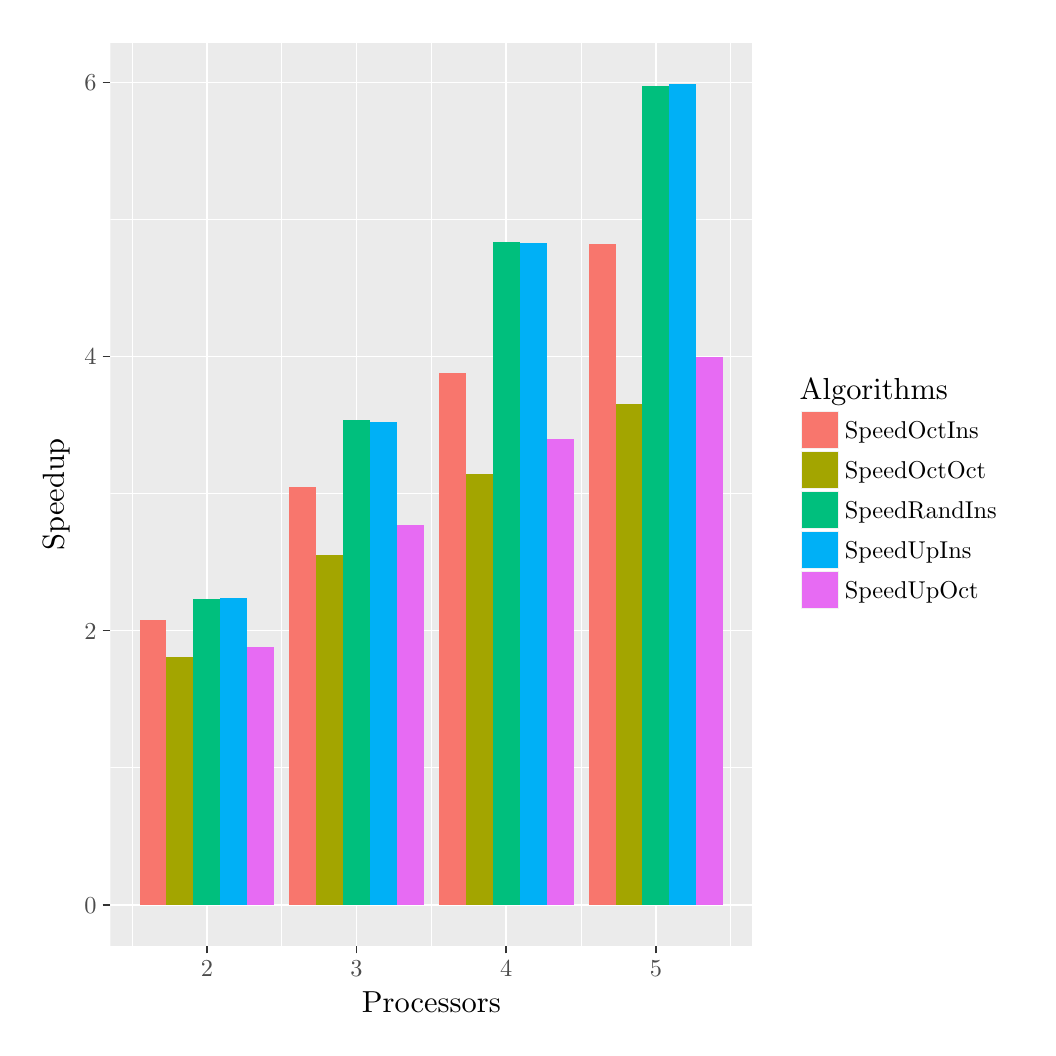
\begin{tikzpicture}[x=1pt,y=1pt]
\definecolor{fillColor}{RGB}{255,255,255}
\path[use as bounding box,fill=fillColor,fill opacity=0.00] (0,0) rectangle (361.35,361.35);
\begin{scope}
\path[clip] (  0.00,  0.00) rectangle (361.35,361.35);
\definecolor{drawColor}{RGB}{255,255,255}
\definecolor{fillColor}{RGB}{255,255,255}

\path[draw=drawColor,line width= 0.6pt,line join=round,line cap=round,fill=fillColor] (  0.00, -0.00) rectangle (361.35,361.35);
\end{scope}
\begin{scope}
\path[clip] ( 29.87, 29.59) rectangle (261.91,355.85);
\definecolor{fillColor}{gray}{0.92}

\path[fill=fillColor] ( 29.87, 29.59) rectangle (261.91,355.85);
\definecolor{drawColor}{RGB}{255,255,255}

\path[draw=drawColor,line width= 0.3pt,line join=round] ( 29.87, 93.94) --
	(261.91, 93.94);

\path[draw=drawColor,line width= 0.3pt,line join=round] ( 29.87,192.99) --
	(261.91,192.99);

\path[draw=drawColor,line width= 0.3pt,line join=round] ( 29.87,292.03) --
	(261.91,292.03);

\path[draw=drawColor,line width= 0.3pt,line join=round] ( 37.71, 29.59) --
	( 37.71,355.85);

\path[draw=drawColor,line width= 0.3pt,line join=round] ( 91.80, 29.59) --
	( 91.80,355.85);

\path[draw=drawColor,line width= 0.3pt,line join=round] (145.89, 29.59) --
	(145.89,355.85);

\path[draw=drawColor,line width= 0.3pt,line join=round] (199.98, 29.59) --
	(199.98,355.85);

\path[draw=drawColor,line width= 0.3pt,line join=round] (254.07, 29.59) --
	(254.07,355.85);

\path[draw=drawColor,line width= 0.6pt,line join=round] ( 29.87, 44.42) --
	(261.91, 44.42);

\path[draw=drawColor,line width= 0.6pt,line join=round] ( 29.87,143.46) --
	(261.91,143.46);

\path[draw=drawColor,line width= 0.6pt,line join=round] ( 29.87,242.51) --
	(261.91,242.51);

\path[draw=drawColor,line width= 0.6pt,line join=round] ( 29.87,341.56) --
	(261.91,341.56);

\path[draw=drawColor,line width= 0.6pt,line join=round] ( 64.76, 29.59) --
	( 64.76,355.85);

\path[draw=drawColor,line width= 0.6pt,line join=round] (118.85, 29.59) --
	(118.85,355.85);

\path[draw=drawColor,line width= 0.6pt,line join=round] (172.94, 29.59) --
	(172.94,355.85);

\path[draw=drawColor,line width= 0.6pt,line join=round] (227.03, 29.59) --
	(227.03,355.85);
\definecolor{fillColor}{RGB}{231,107,243}

\path[fill=fillColor] ( 79.36, 44.42) rectangle ( 89.10,137.60);
\definecolor{fillColor}{RGB}{0,176,246}

\path[fill=fillColor] ( 69.62, 44.42) rectangle ( 79.36,155.21);
\definecolor{fillColor}{RGB}{0,191,125}

\path[fill=fillColor] ( 59.89, 44.42) rectangle ( 69.62,155.00);
\definecolor{fillColor}{RGB}{163,165,0}

\path[fill=fillColor] ( 50.15, 44.42) rectangle ( 59.89,134.00);
\definecolor{fillColor}{RGB}{248,118,109}

\path[fill=fillColor] ( 40.42, 44.42) rectangle ( 50.15,147.22);
\definecolor{fillColor}{RGB}{231,107,243}

\path[fill=fillColor] (133.45, 44.42) rectangle (143.19,181.61);
\definecolor{fillColor}{RGB}{0,176,246}

\path[fill=fillColor] (123.71, 44.42) rectangle (133.45,218.68);
\definecolor{fillColor}{RGB}{0,191,125}

\path[fill=fillColor] (113.98, 44.42) rectangle (123.71,219.57);
\definecolor{fillColor}{RGB}{163,165,0}

\path[fill=fillColor] (104.24, 44.42) rectangle (113.98,170.76);
\definecolor{fillColor}{RGB}{248,118,109}

\path[fill=fillColor] ( 94.51, 44.42) rectangle (104.24,195.50);
\definecolor{fillColor}{RGB}{231,107,243}

\path[fill=fillColor] (187.54, 44.42) rectangle (197.28,212.69);
\definecolor{fillColor}{RGB}{0,176,246}

\path[fill=fillColor] (177.80, 44.42) rectangle (187.54,283.58);
\definecolor{fillColor}{RGB}{0,191,125}

\path[fill=fillColor] (168.07, 44.42) rectangle (177.80,284.00);
\definecolor{fillColor}{RGB}{163,165,0}

\path[fill=fillColor] (158.33, 44.42) rectangle (168.07,200.20);
\definecolor{fillColor}{RGB}{248,118,109}

\path[fill=fillColor] (148.60, 44.42) rectangle (158.33,236.72);
\definecolor{fillColor}{RGB}{231,107,243}

\path[fill=fillColor] (241.63, 44.42) rectangle (251.37,242.32);
\definecolor{fillColor}{RGB}{0,176,246}

\path[fill=fillColor] (231.89, 44.42) rectangle (241.63,341.02);
\definecolor{fillColor}{RGB}{0,191,125}

\path[fill=fillColor] (222.16, 44.42) rectangle (231.89,340.15);
\definecolor{fillColor}{RGB}{163,165,0}

\path[fill=fillColor] (212.42, 44.42) rectangle (222.16,225.51);
\definecolor{fillColor}{RGB}{248,118,109}

\path[fill=fillColor] (202.69, 44.42) rectangle (212.42,283.12);
\end{scope}
\begin{scope}
\path[clip] (  0.00,  0.00) rectangle (361.35,361.35);
\definecolor{drawColor}{gray}{0.30}

\node[text=drawColor,anchor=base east,inner sep=0pt, outer sep=0pt, scale=  0.88] at ( 24.92, 41.39) {0};

\node[text=drawColor,anchor=base east,inner sep=0pt, outer sep=0pt, scale=  0.88] at ( 24.92,140.43) {2};

\node[text=drawColor,anchor=base east,inner sep=0pt, outer sep=0pt, scale=  0.88] at ( 24.92,239.48) {4};

\node[text=drawColor,anchor=base east,inner sep=0pt, outer sep=0pt, scale=  0.88] at ( 24.92,338.53) {6};
\end{scope}
\begin{scope}
\path[clip] (  0.00,  0.00) rectangle (361.35,361.35);
\definecolor{drawColor}{gray}{0.20}

\path[draw=drawColor,line width= 0.6pt,line join=round] ( 27.12, 44.42) --
	( 29.87, 44.42);

\path[draw=drawColor,line width= 0.6pt,line join=round] ( 27.12,143.46) --
	( 29.87,143.46);

\path[draw=drawColor,line width= 0.6pt,line join=round] ( 27.12,242.51) --
	( 29.87,242.51);

\path[draw=drawColor,line width= 0.6pt,line join=round] ( 27.12,341.56) --
	( 29.87,341.56);
\end{scope}
\begin{scope}
\path[clip] (  0.00,  0.00) rectangle (361.35,361.35);
\definecolor{drawColor}{gray}{0.20}

\path[draw=drawColor,line width= 0.6pt,line join=round] ( 64.76, 26.84) --
	( 64.76, 29.59);

\path[draw=drawColor,line width= 0.6pt,line join=round] (118.85, 26.84) --
	(118.85, 29.59);

\path[draw=drawColor,line width= 0.6pt,line join=round] (172.94, 26.84) --
	(172.94, 29.59);

\path[draw=drawColor,line width= 0.6pt,line join=round] (227.03, 26.84) --
	(227.03, 29.59);
\end{scope}
\begin{scope}
\path[clip] (  0.00,  0.00) rectangle (361.35,361.35);
\definecolor{drawColor}{gray}{0.30}

\node[text=drawColor,anchor=base,inner sep=0pt, outer sep=0pt, scale=  0.88] at ( 64.76, 18.58) {2};

\node[text=drawColor,anchor=base,inner sep=0pt, outer sep=0pt, scale=  0.88] at (118.85, 18.58) {3};

\node[text=drawColor,anchor=base,inner sep=0pt, outer sep=0pt, scale=  0.88] at (172.94, 18.58) {4};

\node[text=drawColor,anchor=base,inner sep=0pt, outer sep=0pt, scale=  0.88] at (227.03, 18.58) {5};
\end{scope}
\begin{scope}
\path[clip] (  0.00,  0.00) rectangle (361.35,361.35);
\definecolor{drawColor}{RGB}{0,0,0}

\node[text=drawColor,anchor=base,inner sep=0pt, outer sep=0pt, scale=  1.10] at (145.89,  5.50) {Processors};
\end{scope}
\begin{scope}
\path[clip] (  0.00,  0.00) rectangle (361.35,361.35);
\definecolor{drawColor}{RGB}{0,0,0}

\node[text=drawColor,rotate= 90.00,anchor=base,inner sep=0pt, outer sep=0pt, scale=  1.10] at ( 13.08,192.72) {Speedup};
\end{scope}
\begin{scope}
\path[clip] (  0.00,  0.00) rectangle (361.35,361.35);
\definecolor{fillColor}{RGB}{255,255,255}

\path[fill=fillColor] (273.29,145.30) rectangle (355.85,240.14);
\end{scope}
\begin{scope}
\path[clip] (  0.00,  0.00) rectangle (361.35,361.35);
\definecolor{drawColor}{RGB}{0,0,0}

\node[text=drawColor,anchor=base west,inner sep=0pt, outer sep=0pt, scale=  1.10] at (278.99,226.87) {Algorithms};
\end{scope}
\begin{scope}
\path[clip] (  0.00,  0.00) rectangle (361.35,361.35);
\definecolor{drawColor}{RGB}{255,255,255}
\definecolor{fillColor}{gray}{0.95}

\path[draw=drawColor,line width= 0.6pt,line join=round,line cap=round,fill=fillColor] (278.99,208.80) rectangle (293.44,223.26);
\end{scope}
\begin{scope}
\path[clip] (  0.00,  0.00) rectangle (361.35,361.35);
\definecolor{fillColor}{RGB}{248,118,109}

\path[fill=fillColor] (279.70,209.52) rectangle (292.73,222.55);
\end{scope}
\begin{scope}
\path[clip] (  0.00,  0.00) rectangle (361.35,361.35);
\definecolor{drawColor}{RGB}{255,255,255}
\definecolor{fillColor}{gray}{0.95}

\path[draw=drawColor,line width= 0.6pt,line join=round,line cap=round,fill=fillColor] (278.99,194.35) rectangle (293.44,208.80);
\end{scope}
\begin{scope}
\path[clip] (  0.00,  0.00) rectangle (361.35,361.35);
\definecolor{fillColor}{RGB}{163,165,0}

\path[fill=fillColor] (279.70,195.06) rectangle (292.73,208.09);
\end{scope}
\begin{scope}
\path[clip] (  0.00,  0.00) rectangle (361.35,361.35);
\definecolor{drawColor}{RGB}{255,255,255}
\definecolor{fillColor}{gray}{0.95}

\path[draw=drawColor,line width= 0.6pt,line join=round,line cap=round,fill=fillColor] (278.99,179.90) rectangle (293.44,194.35);
\end{scope}
\begin{scope}
\path[clip] (  0.00,  0.00) rectangle (361.35,361.35);
\definecolor{fillColor}{RGB}{0,191,125}

\path[fill=fillColor] (279.70,180.61) rectangle (292.73,193.64);
\end{scope}
\begin{scope}
\path[clip] (  0.00,  0.00) rectangle (361.35,361.35);
\definecolor{drawColor}{RGB}{255,255,255}
\definecolor{fillColor}{gray}{0.95}

\path[draw=drawColor,line width= 0.6pt,line join=round,line cap=round,fill=fillColor] (278.99,165.44) rectangle (293.44,179.90);
\end{scope}
\begin{scope}
\path[clip] (  0.00,  0.00) rectangle (361.35,361.35);
\definecolor{fillColor}{RGB}{0,176,246}

\path[fill=fillColor] (279.70,166.15) rectangle (292.73,179.19);
\end{scope}
\begin{scope}
\path[clip] (  0.00,  0.00) rectangle (361.35,361.35);
\definecolor{drawColor}{RGB}{255,255,255}
\definecolor{fillColor}{gray}{0.95}

\path[draw=drawColor,line width= 0.6pt,line join=round,line cap=round,fill=fillColor] (278.99,150.99) rectangle (293.44,165.44);
\end{scope}
\begin{scope}
\path[clip] (  0.00,  0.00) rectangle (361.35,361.35);
\definecolor{fillColor}{RGB}{231,107,243}

\path[fill=fillColor] (279.70,151.70) rectangle (292.73,164.73);
\end{scope}
\begin{scope}
\path[clip] (  0.00,  0.00) rectangle (361.35,361.35);
\definecolor{drawColor}{RGB}{0,0,0}

\node[text=drawColor,anchor=base west,inner sep=0pt, outer sep=0pt, scale=  0.88] at (295.25,213.00) {SpeedOctIns};
\end{scope}
\begin{scope}
\path[clip] (  0.00,  0.00) rectangle (361.35,361.35);
\definecolor{drawColor}{RGB}{0,0,0}

\node[text=drawColor,anchor=base west,inner sep=0pt, outer sep=0pt, scale=  0.88] at (295.25,198.55) {SpeedOctOct};
\end{scope}
\begin{scope}
\path[clip] (  0.00,  0.00) rectangle (361.35,361.35);
\definecolor{drawColor}{RGB}{0,0,0}

\node[text=drawColor,anchor=base west,inner sep=0pt, outer sep=0pt, scale=  0.88] at (295.25,184.09) {SpeedRandIns};
\end{scope}
\begin{scope}
\path[clip] (  0.00,  0.00) rectangle (361.35,361.35);
\definecolor{drawColor}{RGB}{0,0,0}

\node[text=drawColor,anchor=base west,inner sep=0pt, outer sep=0pt, scale=  0.88] at (295.25,169.64) {SpeedUpIns};
\end{scope}
\begin{scope}
\path[clip] (  0.00,  0.00) rectangle (361.35,361.35);
\definecolor{drawColor}{RGB}{0,0,0}

\node[text=drawColor,anchor=base west,inner sep=0pt, outer sep=0pt, scale=  0.88] at (295.25,155.19) {SpeedUpOct};
\end{scope}
\end{tikzpicture}
